\newpage
\graphicspath{ {../choicungbi/domino1/} }
\begingroup
\AddToShipoutPicture*{\put(85,605){
\includegraphics[scale=0.85]{../domino1/domino-td.pdf}}}
\centering
\endgroup
\vspace*{25pt}
	
	Bi biết đến trò Domino từ hồi còn nhỏ. Bi thường hay chơi với chị My và các bạn vào mỗi cuối tuần.
	Bộ Domino gồm các quân nhựa (hoặc gỗ) hình chữ nhật, có hai đầu, mỗi đầu có $0$ hoặc $1$ hoặc $2$ hoặc $3$ hoặc $4$ hoặc $5$ hoặc $6$ chấm.
	\begin{figure}[H]
	\centering
	\vspace*{-10pt}
	\captionsetup{labelformat=empty, justification=centering}
	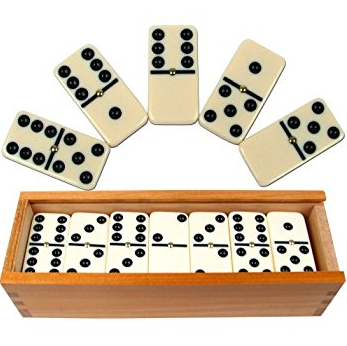
\includegraphics[width=0.34\textwidth]{dom-01}
	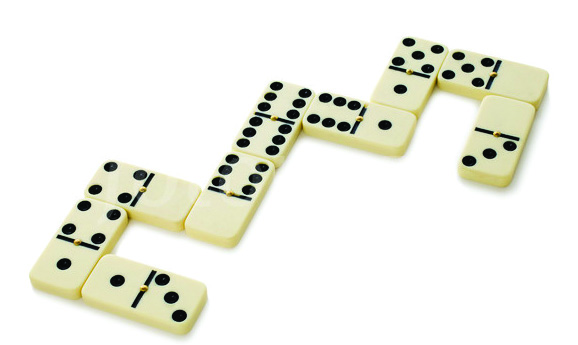
\includegraphics[width=0.48\textwidth]{dom-02}
	\caption{\textit{\small Hình $1.$ \hspace{110pt}Hình $2.$}}
	\vspace*{-15pt}
	\end{figure}
	Trên bàn chơi, luôn có hai hướng để người chơi đặt quân domino nối tiếp vào dãy quân domino đã được đặt trên bàn. Một nước đi hợp lệ là một bước đặt quân domino sao cho đầu quân domino được đặt nối tiếp vào phải có số chấm bằng số chấm ở đầu của quân mà nó nối vào như minh hoạ ở Hình $2$.
	\vskip 0.1cm
	Còn bây giờ, mời Bi và các em, chúng mình cùng khám phá một trò chơi mới, \textit{\textbf{\color{toancuabi}trò chơi Triomino}}, khá giống với Domino, nhưng đặc sắc hơn và phức tạp hơn đáng kể.
	\begin{figure}[H]
		\centering
		\vspace*{-5pt}
		\captionsetup{labelformat=empty, justification=centering}
		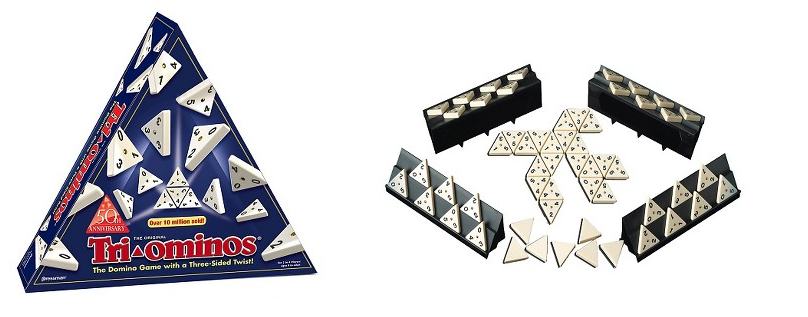
\includegraphics[height=0.25\textwidth]{dom-07}
		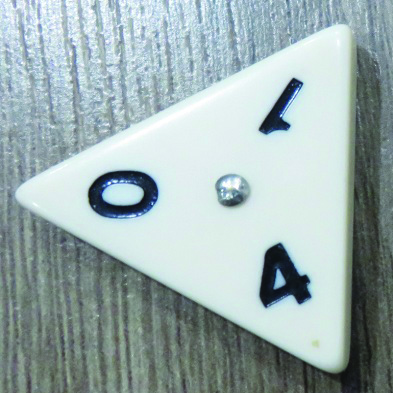
\includegraphics[height=0.25\textwidth]{dom-08}
		\caption{\textit{\small Hình $3.$ \hspace{90pt}Hình $4.$}}
		\vspace*{-5pt}
	\end{figure}
	Quân triomino có hình tam giác đều; ở mỗi góc của tam giác, có ghi một số trong phạm vi từ $0$ đến $5$.
	\vskip 0.1cm
	\newpage
	{\textbf{\color{toancuabi} Cách đi}
	\begin{multicols}{2}
	Trong trò chơi Triomino, một nước đi hợp lệ là một cách ghép hai quân triomino với nhau, sao cho một cạnh của quân triomino này được đặt sát với một cạnh của quân \linebreak triomino kia, đảm bảo hai đỉnh thuộc cạnh này chạm vào hai đỉnh thuộc cạnh kia, đồng thời, hai số ở hai góc tại hai đỉnh chạm nhau
	bằng nhau. Ví dụ, ghép hai quân triomino như ở hình dưới đây là một nước đi hợp lệ:
	\begin{figure}[H]
		\centering
		\vspace*{-5pt}
		\captionsetup{labelformat=empty, justification=centering}
		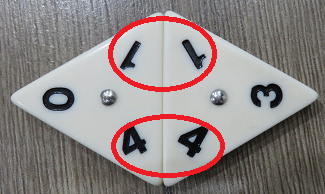
\includegraphics[width=0.48\textwidth]{dom-09}
		\caption{\textit{\small Hình $5.$}}
%		\vspace*{-5pt}
	\end{figure}
	\end{multicols}
	\vspace*{-5pt}
	{\textbf{\color{toancuabi} Câu hỏi $\pmb{1}$:}  % 4/12
	\vskip 0.1cm
	Theo em, các cách ghép hai quân triomino trong các hình dưới đây có phải là những nước đi hợp lệ hay không? Vì sao?
	\begin{figure}[H]
		\centering
		\vspace*{-5pt}
		\captionsetup{labelformat=empty, justification=centering}
		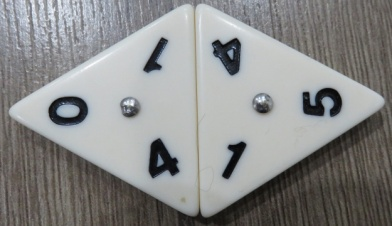
\includegraphics[width=0.3\textwidth]{dom-10a}\quad
		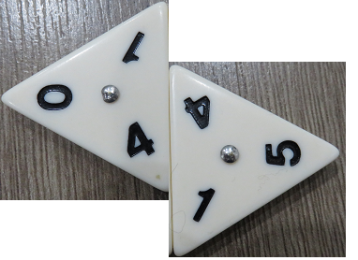
\includegraphics[width=0.3\textwidth]{dom-10b}\quad
		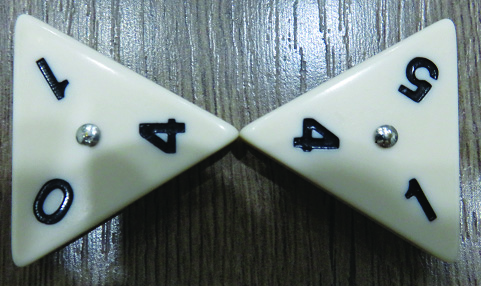
\includegraphics[width=0.3\textwidth]{dom-10c}
		\caption{\textit{\small Hình $a.$ \hspace{70pt}Hình $b.$ \hspace{70pt}Hình $c.$ }}
		\vspace*{-5pt}
	\end{figure}
	{\textbf{\color{toancuabi} Lời giải}   %  4/12
	\vskip 0.1cm
	Trả lời: Cả ba cách ghép trên đều không phải là những nước đi hợp lệ. Cụ thể:
	\vskip 0.1cm
	-- Cách ghép ở Hình $a$ không phải là nước đi hợp lệ, vì hai số ở hai góc tại hai đỉnh chạm nhau không bằng nhau ($1$ không bằng với $4$).
	\vskip 0.1cm
	-- Cách ghép ở Hình $b$ không phải là nước đi hợp lệ, vì không có hai đỉnh nào chạm nhau.
	\vskip 0.1cm
	-- Cách ghép ở Hình $c$ không phải là nước đi hợp lệ, vì không có hai cạnh nào chạm nhau.
	\vskip 0.1cm
	{\textbf{\color{toancuabi} {Điểm cho mỗi lần đi}}   %4/12
	\vskip 0.1cm
	Để cho tiện, chúng mình sẽ ký hiệu $(a, b, c)$ là quân triomino mà ở ba góc của nó có ghi ba số $a, b, c$. Ví dụ, quân triomino ở Hình $6$ dưới đây có ba số ở ba góc là $0, 1, 4$; vì thế, nó được ký hiệu là $(0, 1, 4)$:
	\begin{multicols}{2}
		\begin{figure}[H]
			\centering
			\vspace*{5pt}
			\captionsetup{labelformat=empty, justification=centering}
			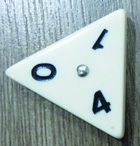
\includegraphics[height=0.19\textwidth]{h4a}
			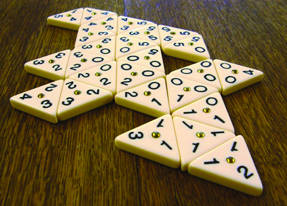
\includegraphics[height=0.19\textwidth]{h5a}
			%\caption{\textit{\small Hình 4}}
			\caption{\textit{\small Hình $6.$ \hspace{50pt}Hình $7.$}}
			\vspace*{-5pt}
		\end{figure}
		\vspace*{-5pt}
		Ở trò chơi Domino, trên bàn chơi lúc nào cũng có hai đầu để đặt quân domino mới. Còn ở trò chơi Triomino thì sao nhỉ? Sau một số nước đi hợp lệ, liệu trên bàn chơi có bao nhiêu vị trí để đặt quân \linebreak triomino tiếp theo?
	\end{multicols}
	\textbf{\color{toancuabi}Câu hỏi $\pmb{2}$:}
	\vskip 0.1cm
	Trên bàn chơi Triomino, có thể có bao nhiêu vị trí để đặt quân triomino tiếp theo?
	\vskip 0.2cm
	\hspace*{20pt}(A)  $1.$ \hspace*{50pt}(B)  $2.$
	\hspace*{50pt}(C)  $3.$ \hspace*{50pt}(D)  nhiều.
	\vskip 0.2cm
	Các em hãy quan sát Hình $7$ để tìm ra câu trả lời.
	\begin{multicols}{2}
	Để chơi Triomino, các em không những phải nhớ quy tắc ghép hai quân triomino với nhau, mà còn phải biết cộng nữa đấy; vì ở trò chơi này có luật cộng điểm. Điểm người chơi có được sau mỗi nước đi hợp lệ là tổng của các số ghi trên quân triomino mà người chơi đó vừa đặt. Ví dụ, ở một nước đi hợp lệ nào đó, em đã đặt quân triomino $(1, 3, 4)$ lên bàn chơi, thế thì em sẽ được cộng thêm vào quỹ điểm của mình
	\vskip 0.1cm
	\centerline{$1+3+4=8$ (điểm).}
	\vskip 0.1cm
	\begin{figure}[H]
		\vspace*{-5pt}
		\centering
		\captionsetup{labelformat=empty, justification=centering}
		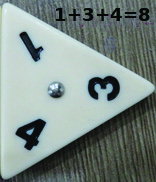
\includegraphics[width=0.3\textwidth]{h6-fix}
		\caption{\textit{\small Hình 8}}
		\vspace*{-5pt}
	\end{figure}
	\end{multicols}
